\chapter{Images}

\begin{figure}[h]
    \centering
    
\includegraphics[width=0.6\textwidth]{data/png/3d}
    \caption[3D view of segmented skull data set]
{
3D View of segmented data set.
VTK viewer used to visualize the data set.
On the left part there is parietal part of the skull.
This part is quite well segmented as illustrate Figure \ref{fg:parietalSlicesSegmentation}
The segmentation of the front skull part (on the right side) is poor due to leaking through eye sockets (see Figure \ref{fg:frontSlicesSegmentation}).
}
    \label{fg:series3d}
\end{figure}

\begin{figure}
    \centering
    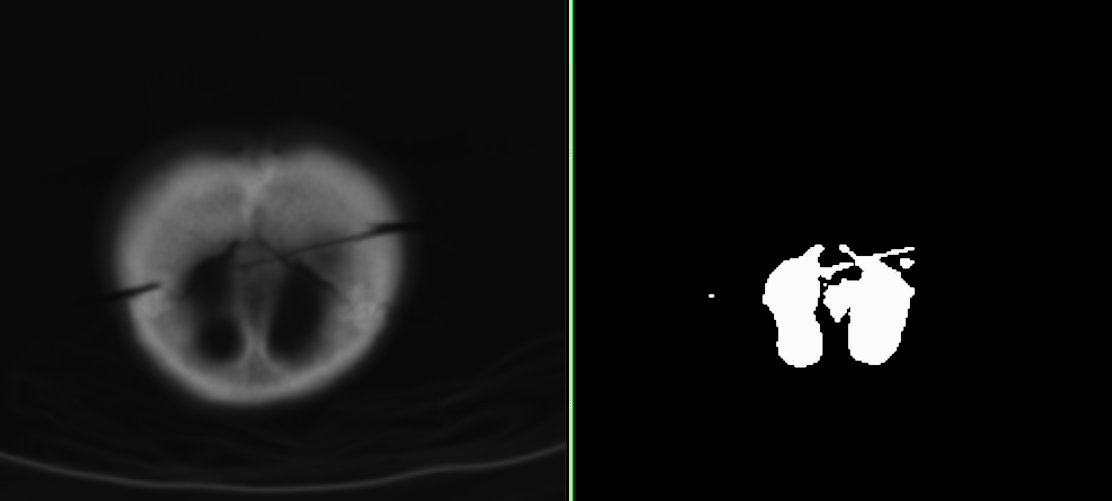
\includegraphics[width=0.95\textwidth]{data/png/2}
    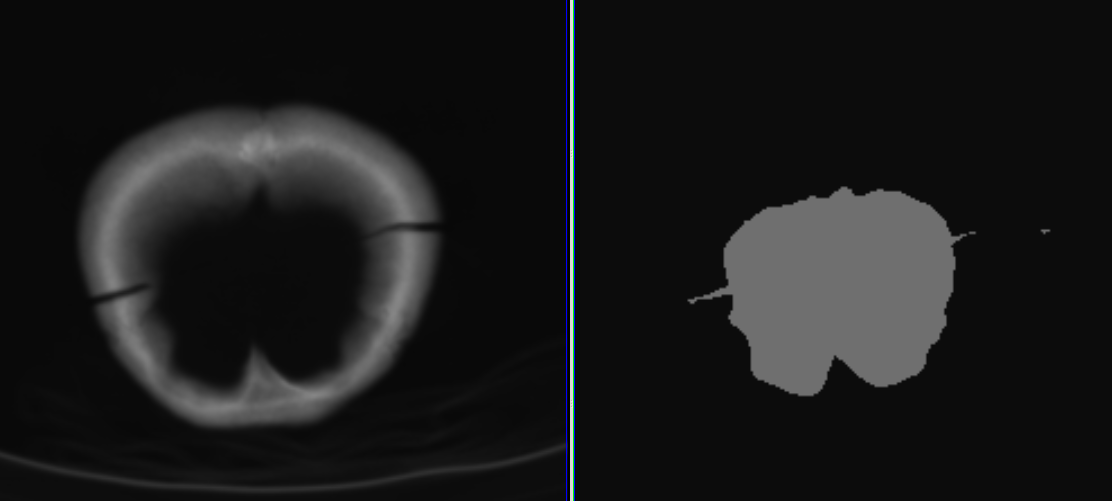
\includegraphics[width=0.95\textwidth]{data/png/4}
    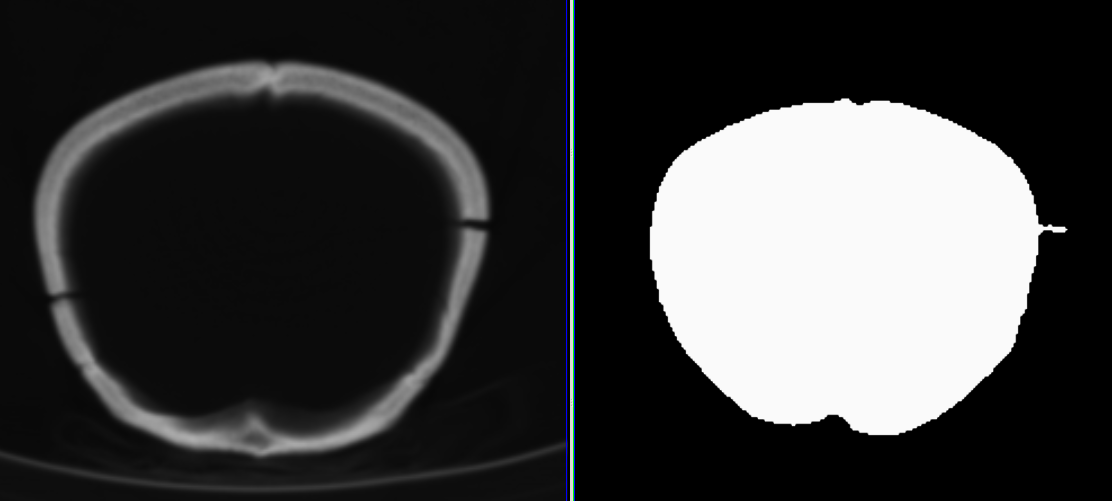
\includegraphics[width=0.95\textwidth]{data/png/7}
    \caption[Result of segmentation of parietal part of a skull]
{
Here is illustration of segmentation of the parental part of a skull.
Cavities that should be segmented are small enough to let the level set reach all the edges.
The segmentation has not completely leaked through the holes on both sides due to curvature term.
But if the holes were wider there would be leakings similar to the ones showed on following figures.
}
    \label{fg:parietalSlicesSegmentation}
\end{figure}

\begin{figure}
    \centering
    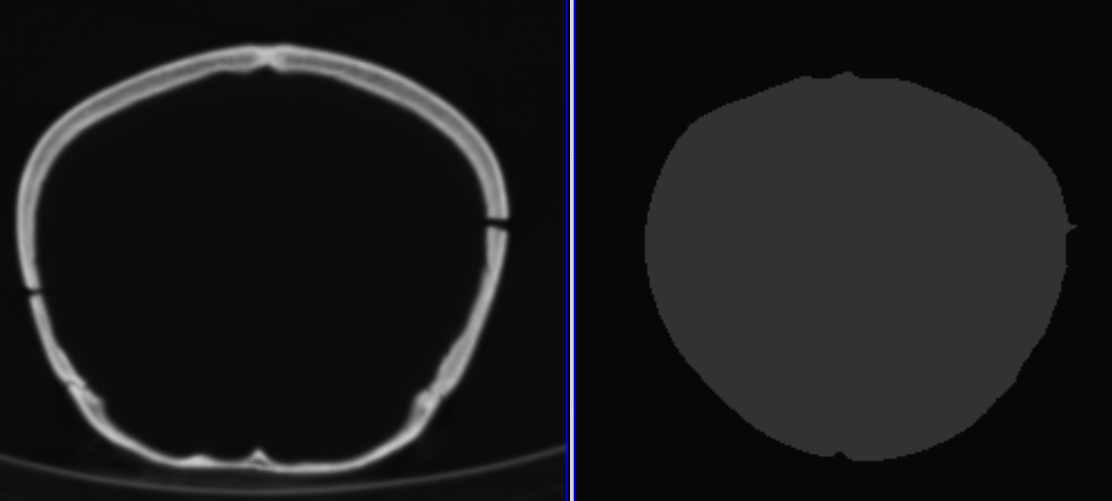
\includegraphics[width=0.95\textwidth]{data/png/12}
    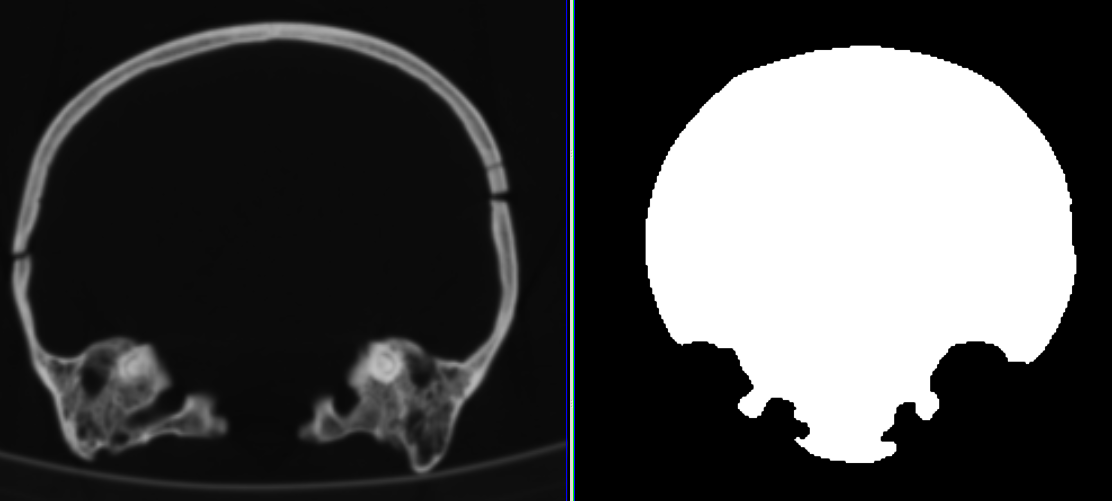
\includegraphics[width=0.95\textwidth]{data/png/17}
    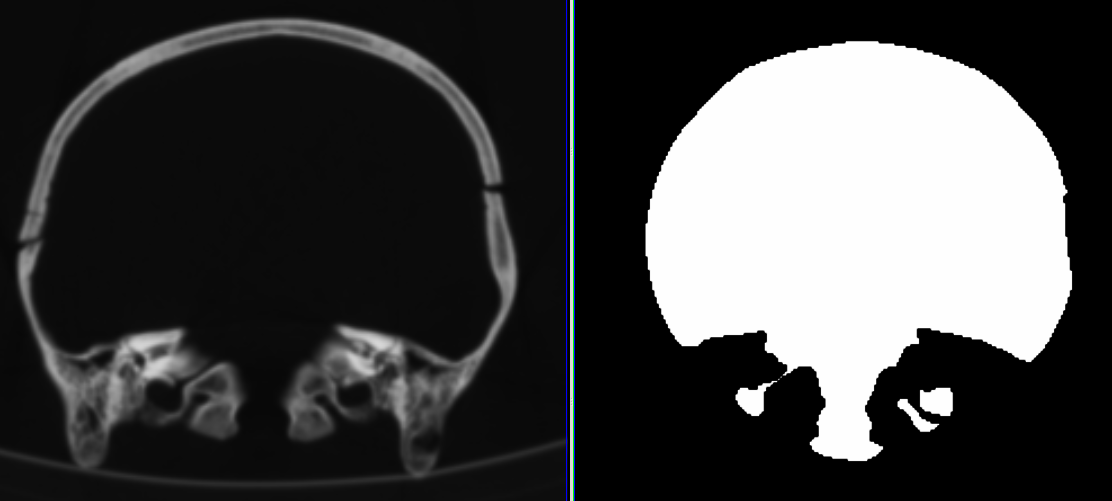
\includegraphics[width=0.95\textwidth]{data/png/18}
    \caption[Result of segmentation middle slices of the skull data set]
{
This image set shows segmentation of middle slices of the skull data set.
Some edges are reached by the level set (on the right side of the skull mostly) while some are not.
This is caused by insufficient of algorithm iterations (500) or improper initial level set placement.
It proves that result is highly initial parameters setting sensitive.
}
    \label{fg:middleSlicesSegmentation}
\end{figure}

\begin{figure}
    \centering
    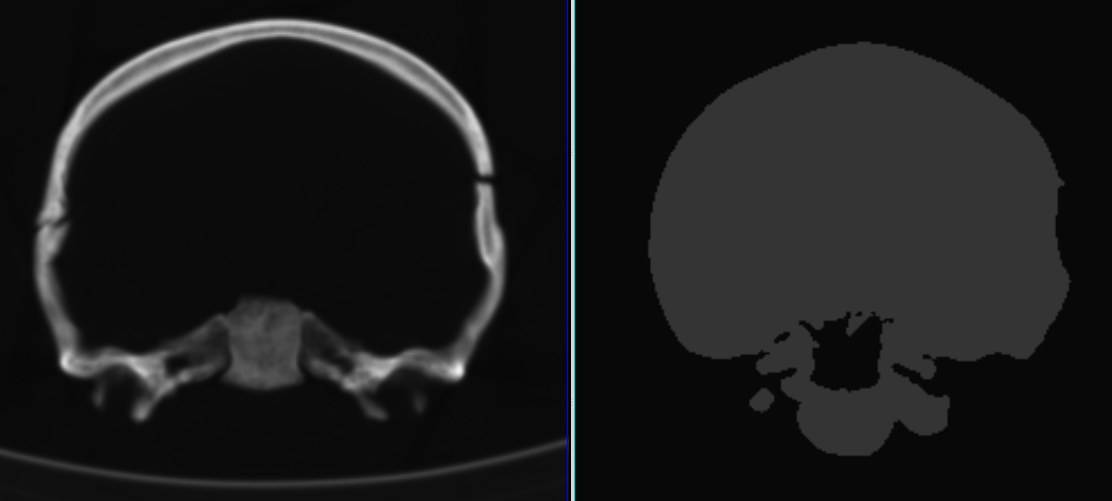
\includegraphics[width=0.95\textwidth]{data/png/20}
    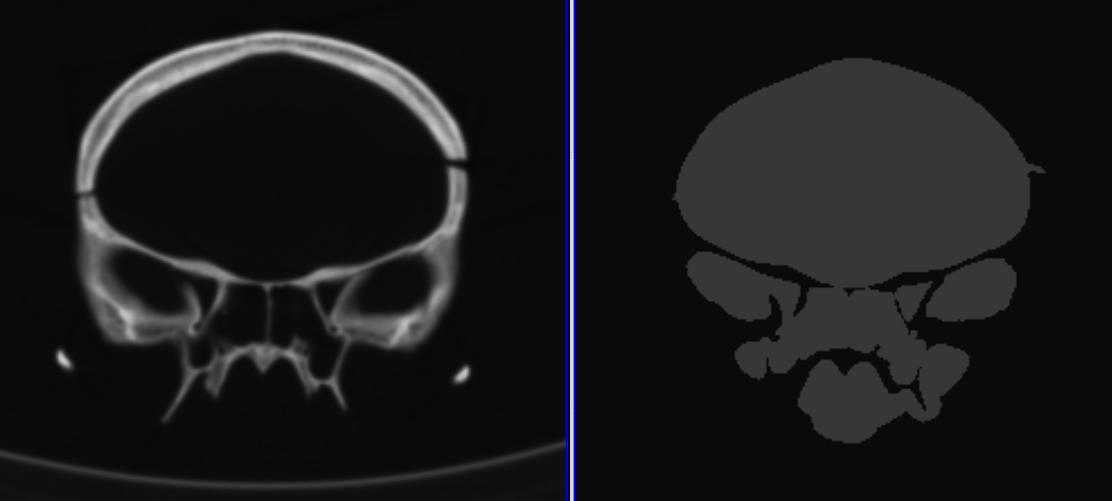
\includegraphics[width=0.95\textwidth]{data/png/23}
    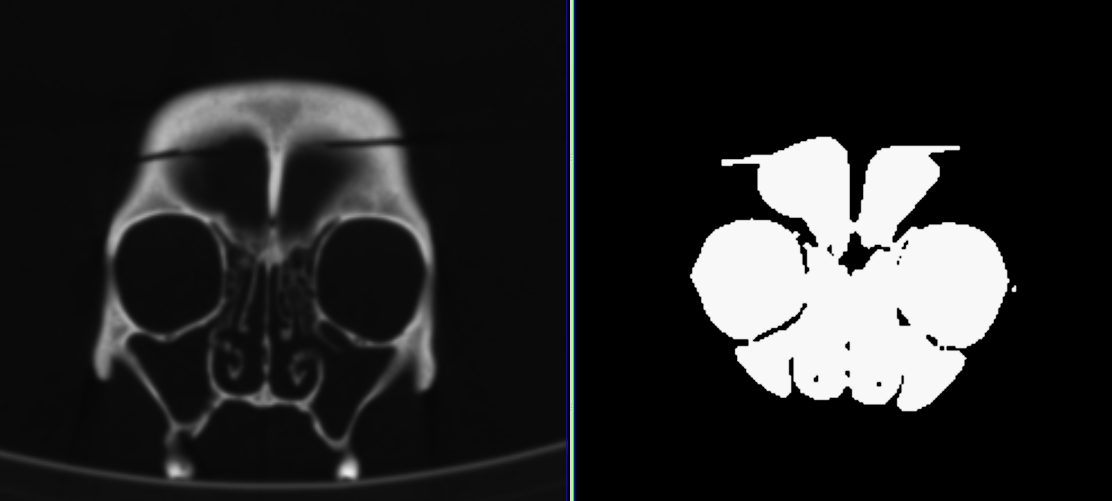
\includegraphics[width=0.95\textwidth]{data/png/27}
    \caption[Result of segmentation front slices of the skull data set]
{
These three images illustrate the leaking of level set through throat hole, cavities near nose and eye sockets.
}
    \label{fg:frontSlicesSegmentation}
\end{figure}

\begin{figure}
    \centering
    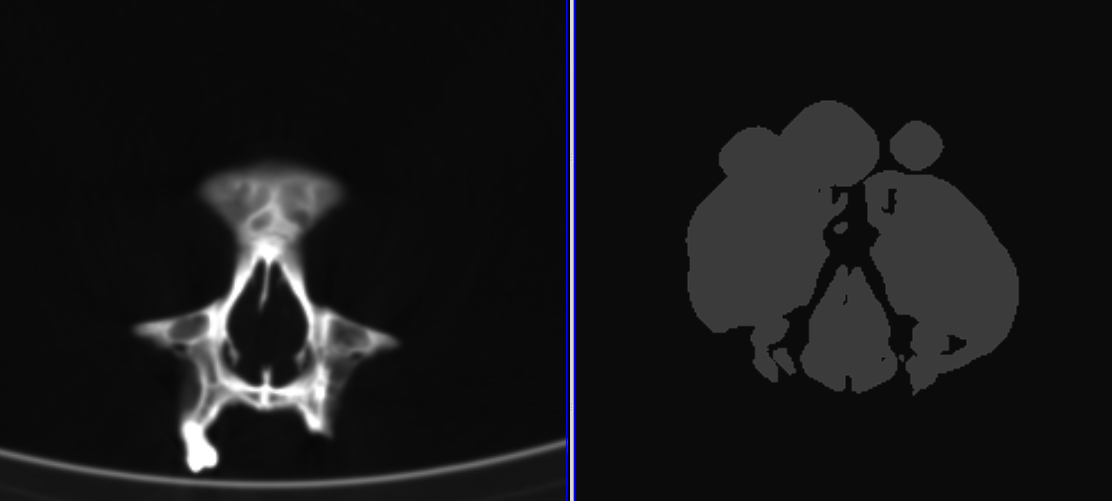
\includegraphics[width=0.95\textwidth]{data/png/29}
    \caption[Result of segmentation of slices near nose]{
This slice is really poorly segmented due the leaking of level set through previous slices (see Figure \ref{fg:frontSlicesSegmentation}).
}
    \label{fg:noseSlicesSegmentation}
\end{figure}
